\documentclass{beamer}

\usepackage[utf8]{inputenc} 
\usepackage[T1]{fontenc}
\usepackage{lmodern}
\usepackage{graphicx}
\usepackage[french]{babel}

\usetheme{Frankfurt}

\addtobeamertemplate{navigation symbols}{\usebeamerfont{footline}%
	\usebeamercolor[fg]{footline}
	\hspace{1em}
	\insertframenumber/\inserttotalframenumber}

\begin{document}

\AtBeginSection[]{
	
	\begin{frame}
	
	\tableofcontents[currentsection]
	
	\end{frame} 

}

\title[Plate-forme d'acquisition multiflux TV Web]{Plate-forme d'acquisition et de formatage temps réel multiflux TV Web}
\subtitle{Soutenance finale de PR\&D}
\author{Romain ROUSSEAU}
\institute{Polytech Tours}
\date{\today}

\begin{frame}[plain]
	\maketitle
\end{frame}

\begin{frame}

\frametitle{Sommaire}

\tableofcontents


\end{frame}

%-------------------------



\section[Contexte et objectifs]{Rappel du contexte et des objectifs}

\begin{frame}
\frametitle{Contexte du projet}

L'analyse temps réel de flux fait l'objet d'enjeux majeurs et peut être utilisé dans de nombreux domaines.

\begin{itemize}
	\item La propriété intellectuelle
	\item La recommandation de vidéo
	\item Le contrôle des vidéos, pour la publicité par exemple
	\item et bien d'autres...
\end{itemize}

\end{frame}

\begin{frame}
\frametitle{Objectifs}

Développer un programme pilote d'acquisition multi-flux TV Web garantissant une synchronisation.

\end{frame}

\begin{frame}
\frametitle{Gestion du projet à l'issue de PR\&D 1}

Passage vers une méthode Agile adaptée avec sprint durant 2 à 3 semaines:

\begin{description}
	\item[Sprint 1]: retour sur la veille technologique et les spécifications
	\item[Sprint 2]: étude sur les chaînes de TV sur internet
	\item[Sprint 3]: développement de la plate-forme
	\item[Sprint 4]: finalisation du rapport
\end{description}


\end{frame}


%----------------------------
\section{Description du programme}

\begin{frame}

\frametitle{Description du programme}

Jar exécutable utilisable en ligne de commande avec un fichier texte contenant les chaînes souhaitées.
\bigbreak
Nécessite trois installations:
\begin{itemize}
	\item Java 8
	\item VLC
	\item Streamlink
\end{itemize}

\end{frame}


\begin{frame}
\frametitle{Fichier texte}

\begin{figure}
	\includegraphics[scale=0.75]{images/textfile}
\end{figure}

\end{frame}

\begin{frame}
\frametitle{Affichage des flux}

\begin{figure}
	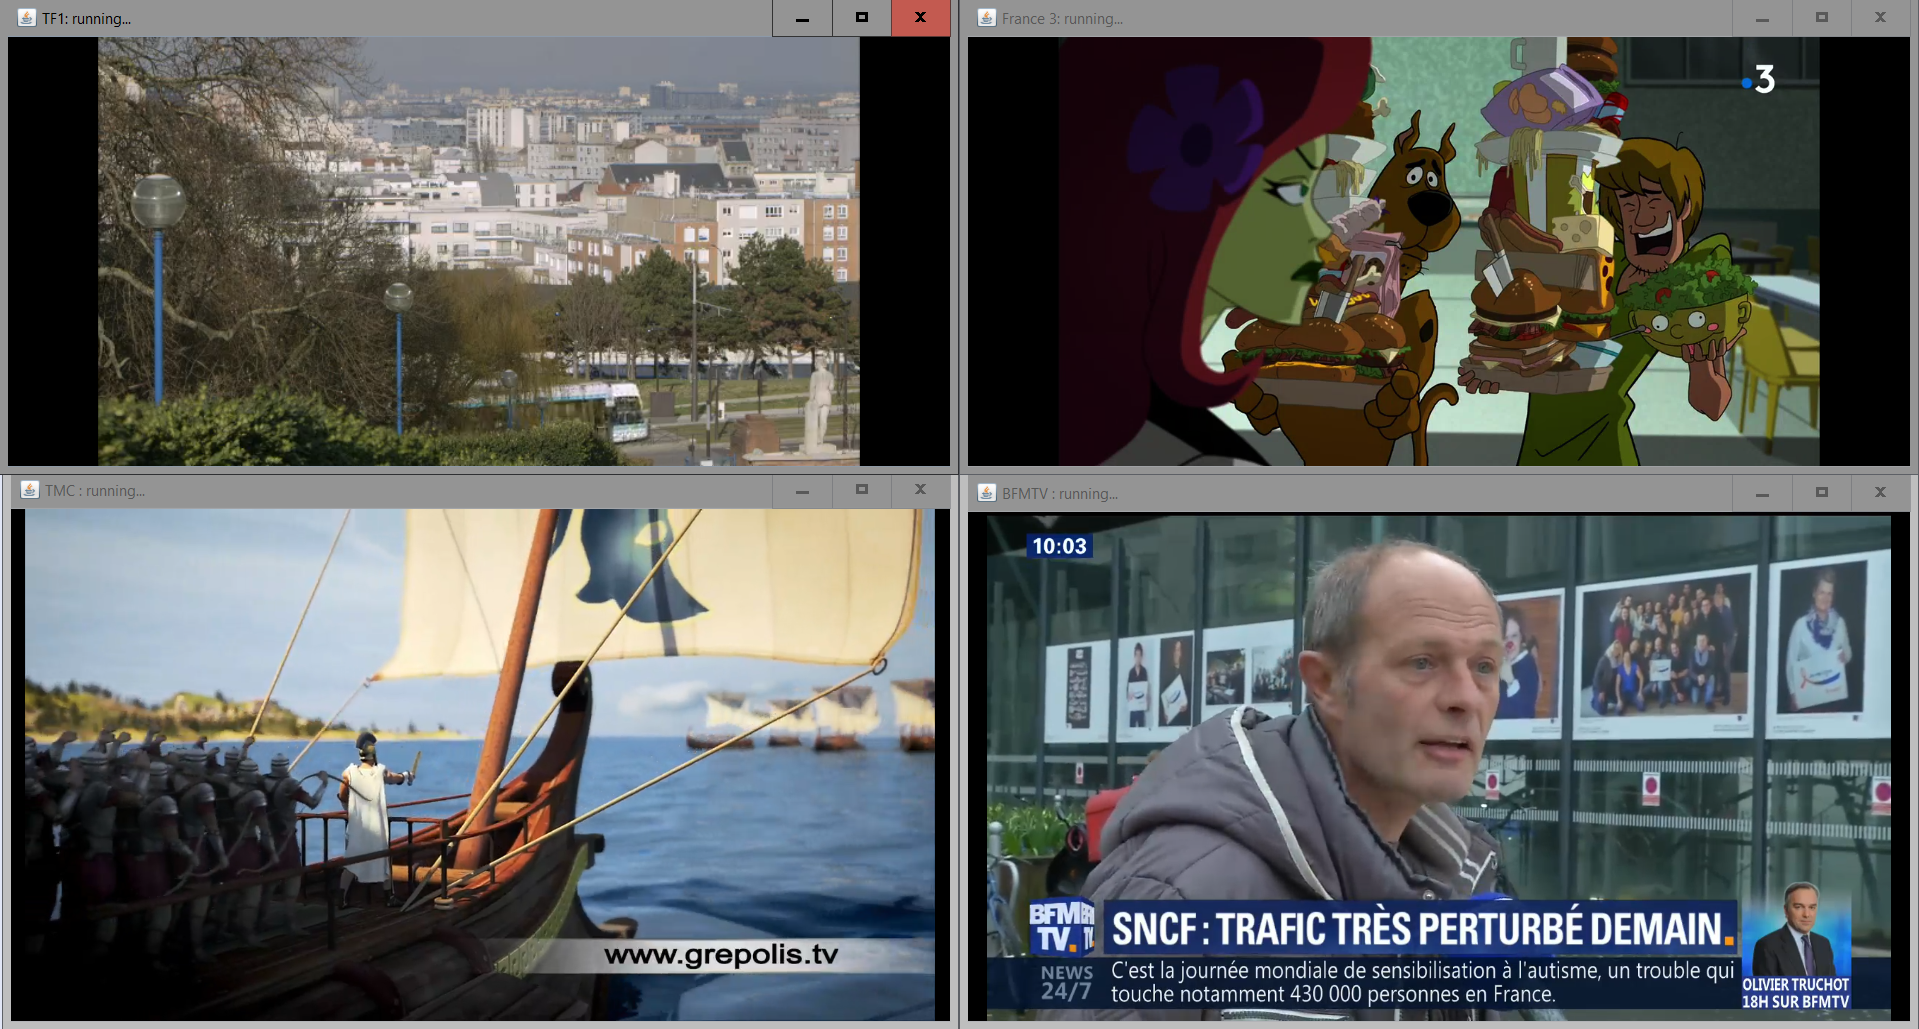
\includegraphics[scale=0.25]{images/affichageFlux}
\end{figure}

\end{frame}

%----------------------------

\section{Explications du code}

\begin{frame}
\frametitle{Structure}

Structure MVC (Modèle, vue, contrôleur): 

\begin{figure}
	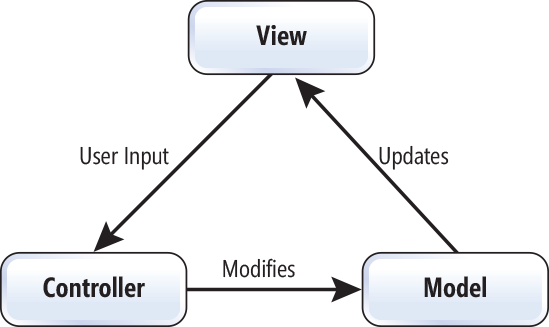
\includegraphics[scale=0.5]{images/mvc}
\end{figure}

\end{frame}

\begin{frame}
\frametitle{Structure}

Classes principales:
\begin{description}
	\item[MainController] : lit le fichier texte et détermine les chaînes à lancer
	\item[StreamController] : lance Streamlink et l'affichage
	\item[StreamView] : affiche les flux sur des fenêtres Java
	\item[TextInputStreamController] : observeur
\end{description}

\end{frame}

\begin{frame}
\frametitle{Structure}

Implémentation d'un pattern Observer pour détecter lorsque Streamlink est prêt. 

\begin{figure}
	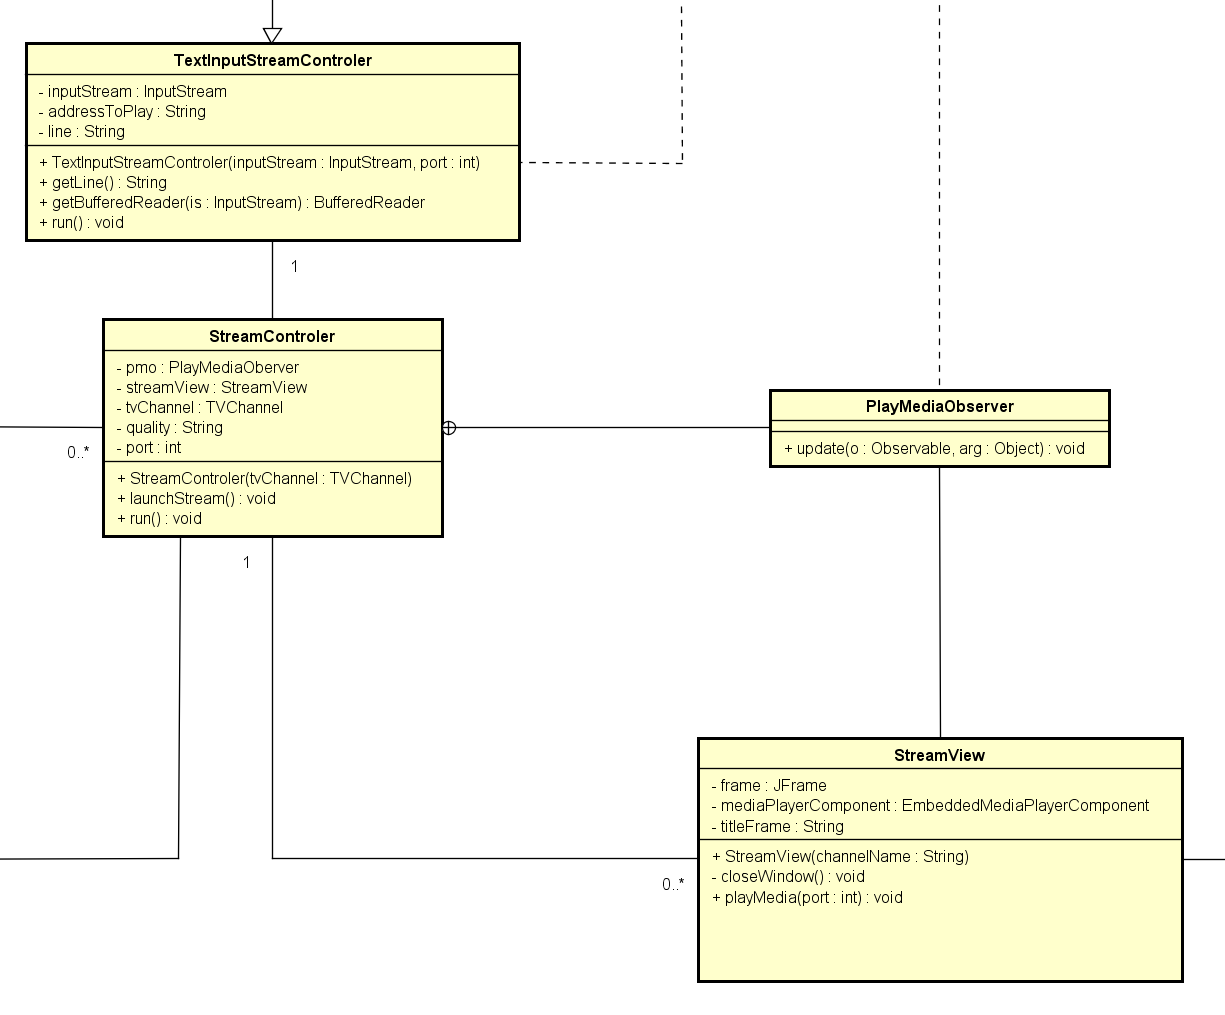
\includegraphics[scale=0.25]{images/ObserverDiag}
\end{figure}

\end{frame}


\begin{frame}
\frametitle{Fonctionnement des threads}

\begin{figure}
	\includegraphics[scale=0.25]{images/seqdiag}
\end{figure}

\end{frame}

%--------------------------

\section{Tests de charges}

\begin{frame}
\frametitle{Tests de charges}

Débit moyen estimé pour un stream en 720p : 1.2 Mbps
\bigbreak
Débit moyen estimé pour 7 streams de qualité moyenne (520p) : 12.5 Mbps
\end{frame}

\begin{frame}
\frametitle{Tests de charges}

Premier test en Wi-fi sur réseau domestique:

Limitation réseau: 7 chaînes en simultané maximum
\bigbreak

Test sur machine virtuelle et réseau de l'école:

Limitation matérielle: 7 chaînes en simultané maximum

\end{frame}


%--------------------------

\section{Qualité de code}

\begin{frame}
\frametitle{Qualité de code}
	\begin{itemize}
		\item Utilisation de logs avec slf4j
		\item Documentation avec Javadoc
		\item Utilisation de Sonar 
	\end{itemize}
\end{frame}


\begin{frame}
\frametitle{SonarQube et SonarLint}

\begin{figure}
	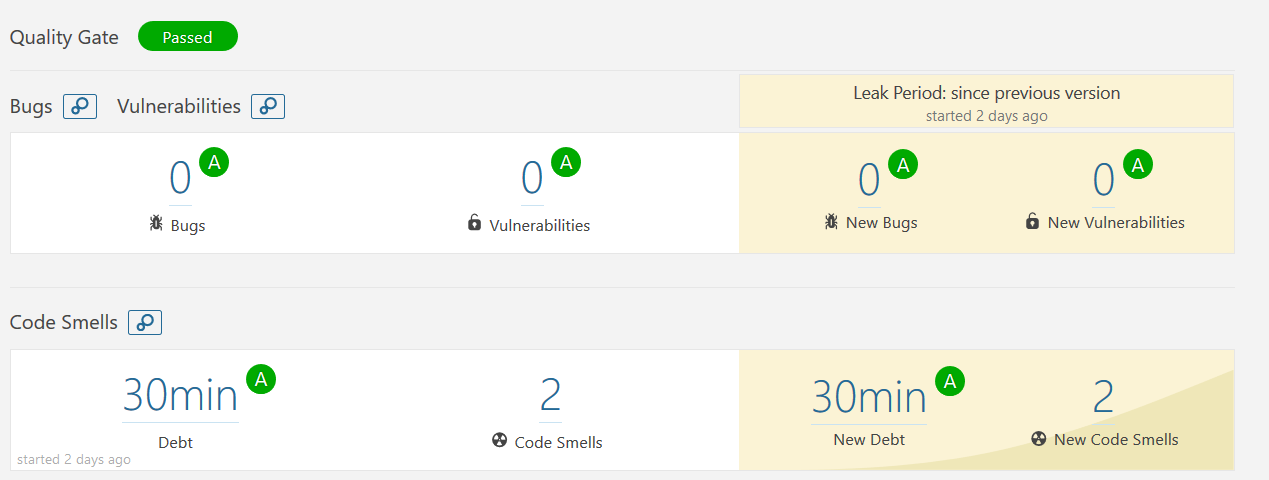
\includegraphics[scale=0.40]{images/sonarresult}
\end{figure}

\end{frame}

%--------------------------
\section*{Conclusion}

\begin{frame}
\frametitle{Améliorations à prévoir}

\begin{itemize}
	\item Ajout d'une interface graphique
	\item Tester sur une machine plus puissante
	\item Passer de VLCJ à VLCJ-pro ou une autre bibliothèque
\end{itemize}

\end{frame}

\begin{frame}
\frametitle{Conclusion}

Projet récupérable sur GitHub : \url{https://github.com/RomainR37/streamPlatform}
\bigbreak

Guide d'utilisation accessible sur le dépôt.

\end{frame}


\end{document}